\documentclass[12pt]{article}
%\documentstyle[12pt]{article}
\setlength{\oddsidemargin}{0in}
\setlength{\evensidemargin}{0in}
\setlength{\textwidth}{6.5in}
\setlength{\topmargin}{-.3in}
\setlength{\textheight}{9in}
\pagestyle{empty}

\usepackage[super]{nth}
\usepackage{amsmath}
\usepackage{csquotes}
\usepackage{physics}
\usepackage{graphicx}% Include figure files
\usepackage{dcolumn}% Align table columns on decimal point
\usepackage{bm}
\usepackage{subfig}

\begin{document}

\begin{center}
{\Large Doppler-Free Saturated Absorption Spectroscopy} \\
{\Large Lab Report} \\[.3in]
{\large Bj\"{o}rn Sumner and Benjamin Crane} \\
{13 Feb 2018}
\end{center}

\section*{Motivation and Context}

The atomic hyperfine structure arises from the interaction of the nuclear and electron magnetic moments.  This structure is responsible for many technological achievements, including the development of atomic clocks.  In fact, the SI second is defined by counting the number of transitions between two hyperfine states in the cesium 133 atom \cite{NISTsec}.  Additionally, the famous 21-cm line in astronomy is generated by a hyperfine transition in interstellar hydrogen\cite{21cmPred}.

The measurement of hyperfine splittings can be performed by using Doppler-Free Saturated Absorption Spectroscopy.  We will use this technique to measure the splittings of several hyperfine structures of Rubidium.

\section*{Physics and Predictions}

\subsection*{Atomic Spectra}
Rubidium is a hydrogen-like atom with a single $5s^1$ electron in its outer shell.  This electron gives rise to the two term states we will be interested in: $5^2\text{S}_{1/2}$ and $5^2\text{P}_{3/2}$.  There are two naturally occurring isotopes of Rubidium: $72\%$ abundant ${}^{85}\text{Rb}$ with spin number $I=5/2$ and $28\%$ abundant ${}^{87}\text{Rb}$ with $I = 3/2$.
The Hamiltonian describing the atom is given by
$$
H = \frac{p^2}{2m} - \frac{Z_{eff} e^2}{4 \pi \epsilon_0 r} + \zeta(r) \vec{L}\cdot \vec{S} + \alpha \vec{J}\cdot \vec{I} + \frac{\beta}{2I(2I-1)J(2J-1)}\left[3(\vec{I}\cdot \vec{J})^2 + \frac{3}{2}(\vec{I}\cdot \vec{J}) - I(I+1)J(J+1)\right]
$$

$\frac{p^2}{2m}$ contains the kinetic energy term and $- \frac{Z_{eff} e^2}{4 \pi \epsilon_0 r}$ the standard Coulomb attractive potential.  $\zeta(r) \vec{L}\cdot \vec{S}$ is the spin orbit coupling term, which gives rise to the broad term states such as $5^2\text{S}_{1/2}$ and $5^2\text{P}_{3/2}$.  The transition between these states is $780\,\text{nm}$.  The final two terms result from the hyperfine interaction.  The former term is the hyperfine interaction between the magnetic dipole of the nucleus and electron, while the latter comes from the nuclear electric quadrupole.  These two terms will produce the hyperfine states we will explore in this lab, and we label these states by their quantum number $F$, the magnitude of the total angular momentum $\vec{F} = \vec{J} + \vec{I}$.  The possible quantum numbers vary from $\rvert J-I\rvert$ to $J+I$.  These energy levels are shown in figure \ref{fig:RbEnergy}.  In this lab, we will look at ${}^{85}\text{Rb}$ transitions from $5^2\text{S}_{1/2}\,\text{F}=3$ to $5^2\text{P}_{3/2}\, \text{F'}=1,2,3,4$ and ${}^{87}\text{Rb}$ transitions from $5^2\text{S}_{1/2}\,\text{F}=2$ to $5^2\text{P}_{3/2}\, \text{F'}=0,1,2,3$.



\subsection*{Doppler Broadening}

The spectra given in the previous section are obtained from a description of nature in the atom's frame of reference with no external effects.  However, real Rubidium atoms are subject to thermal motion, and as such these spectral lines will undergo broadening owing to the motion of the atoms relative to the laser.  Atoms moving toward the laser will `see' radiation blueshifted, and so absorption will only occur if the incoming photons are of a lower frequency than predicted by the spectra in figure \ref{fig:RbEnergy}.  Similarly, atoms moving away from the laser will absorb photons of higher frequency.  Because the velocity of these atoms follows the Maxwell distribution, it can be expected that the spectral lines will similarly follow such a distribution.  It can be shown that the half width of these distributions is given by 
$$\Delta \nu_{1/2} = 2\frac{\nu_0}{c}\sqrt{\frac{2kT}{M}\ln(2)}$$

where $\nu_0$ is the rest frame atomic resonance, $M$ is the mass of the atom and $T$ is the temperature of the sample.

We can use this to predict the expected half width of the D2 lines of ${}^{85}\text{Rb}$ and ${}^{87}\text{Rb}$:

These broadened spectra mask the hyperfine structure of the atoms, and so we must use Doppler-Free Saturated Absorption Spectroscopy to tease out these individual spectra.

\begin{figure}%
	\centering
	\subfloat[${}^{85}\text{Rb}$\cite{steck85Rb}]{{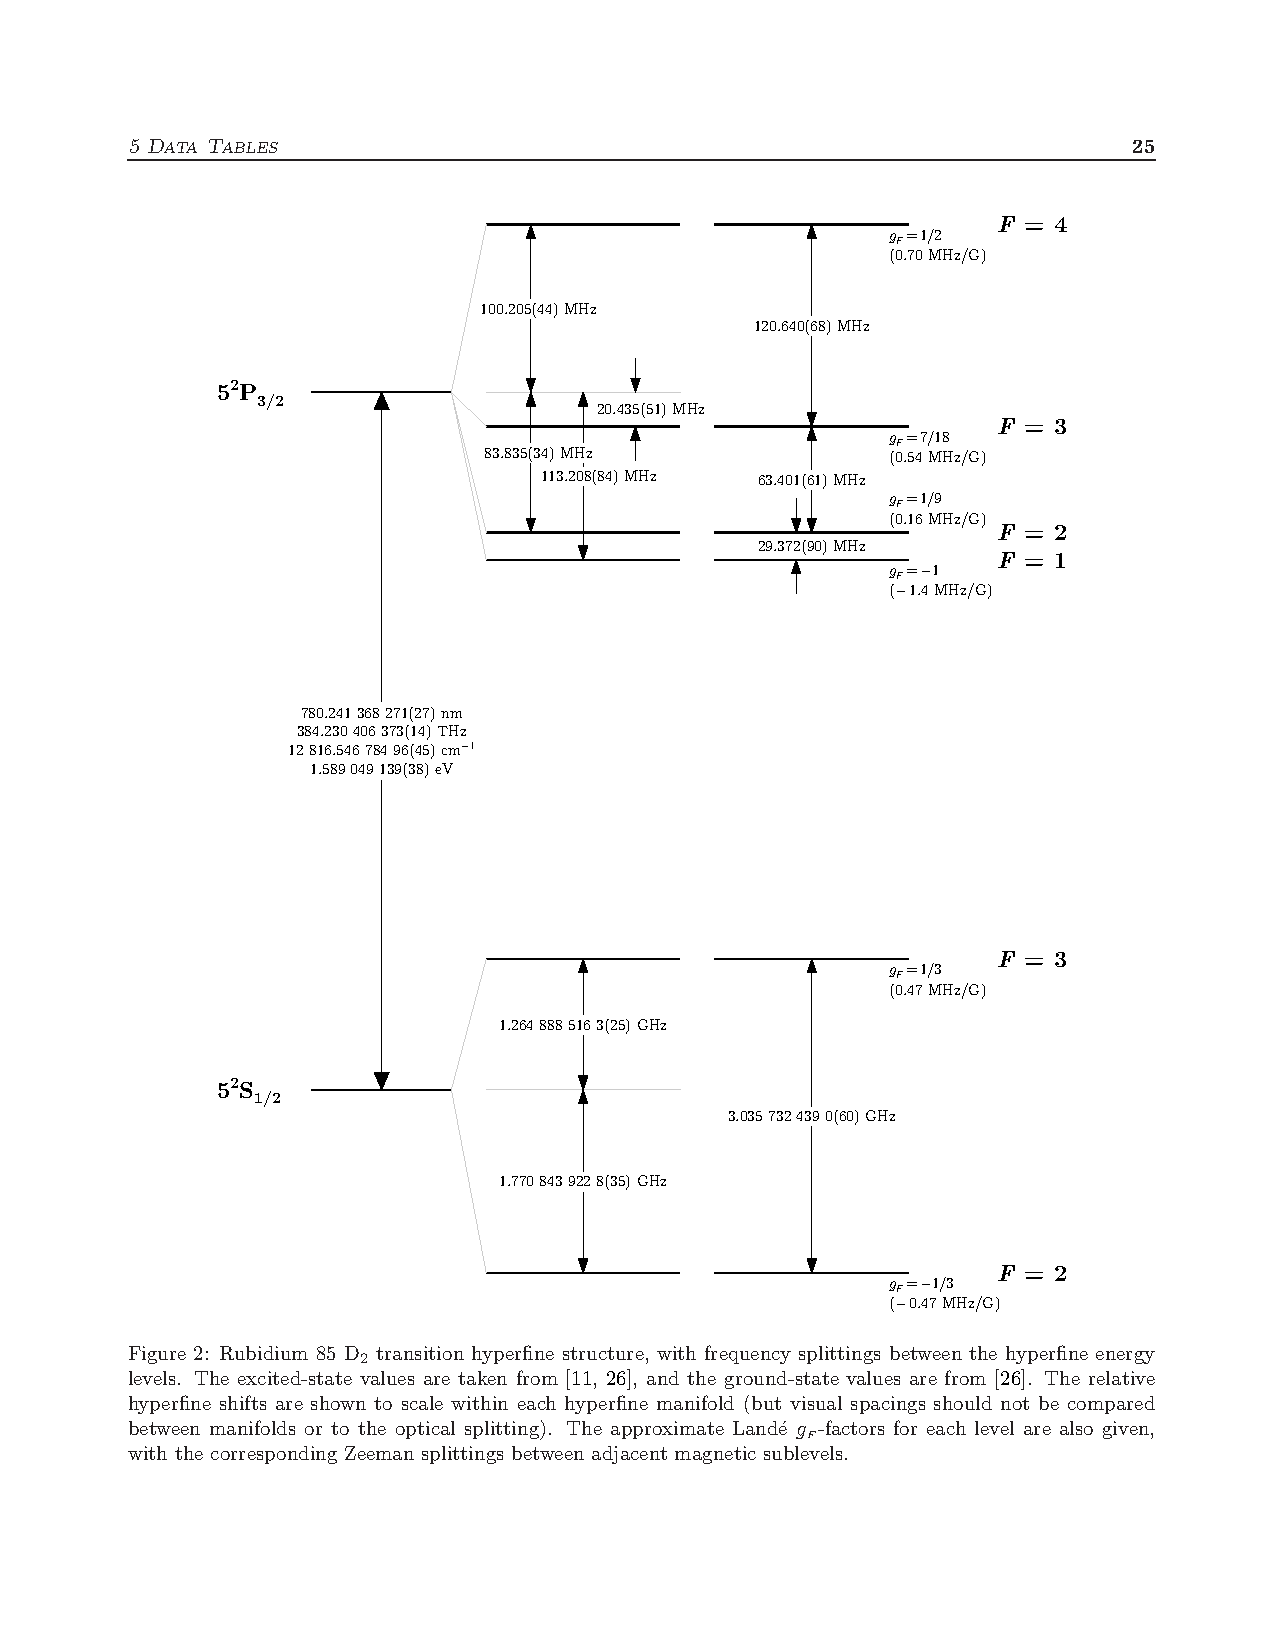
\includegraphics[width=8cm]{85D2.pdf} }}%
	\,
	\subfloat[${}^{87}\text{Rb}$\cite{steck87Rb}]{{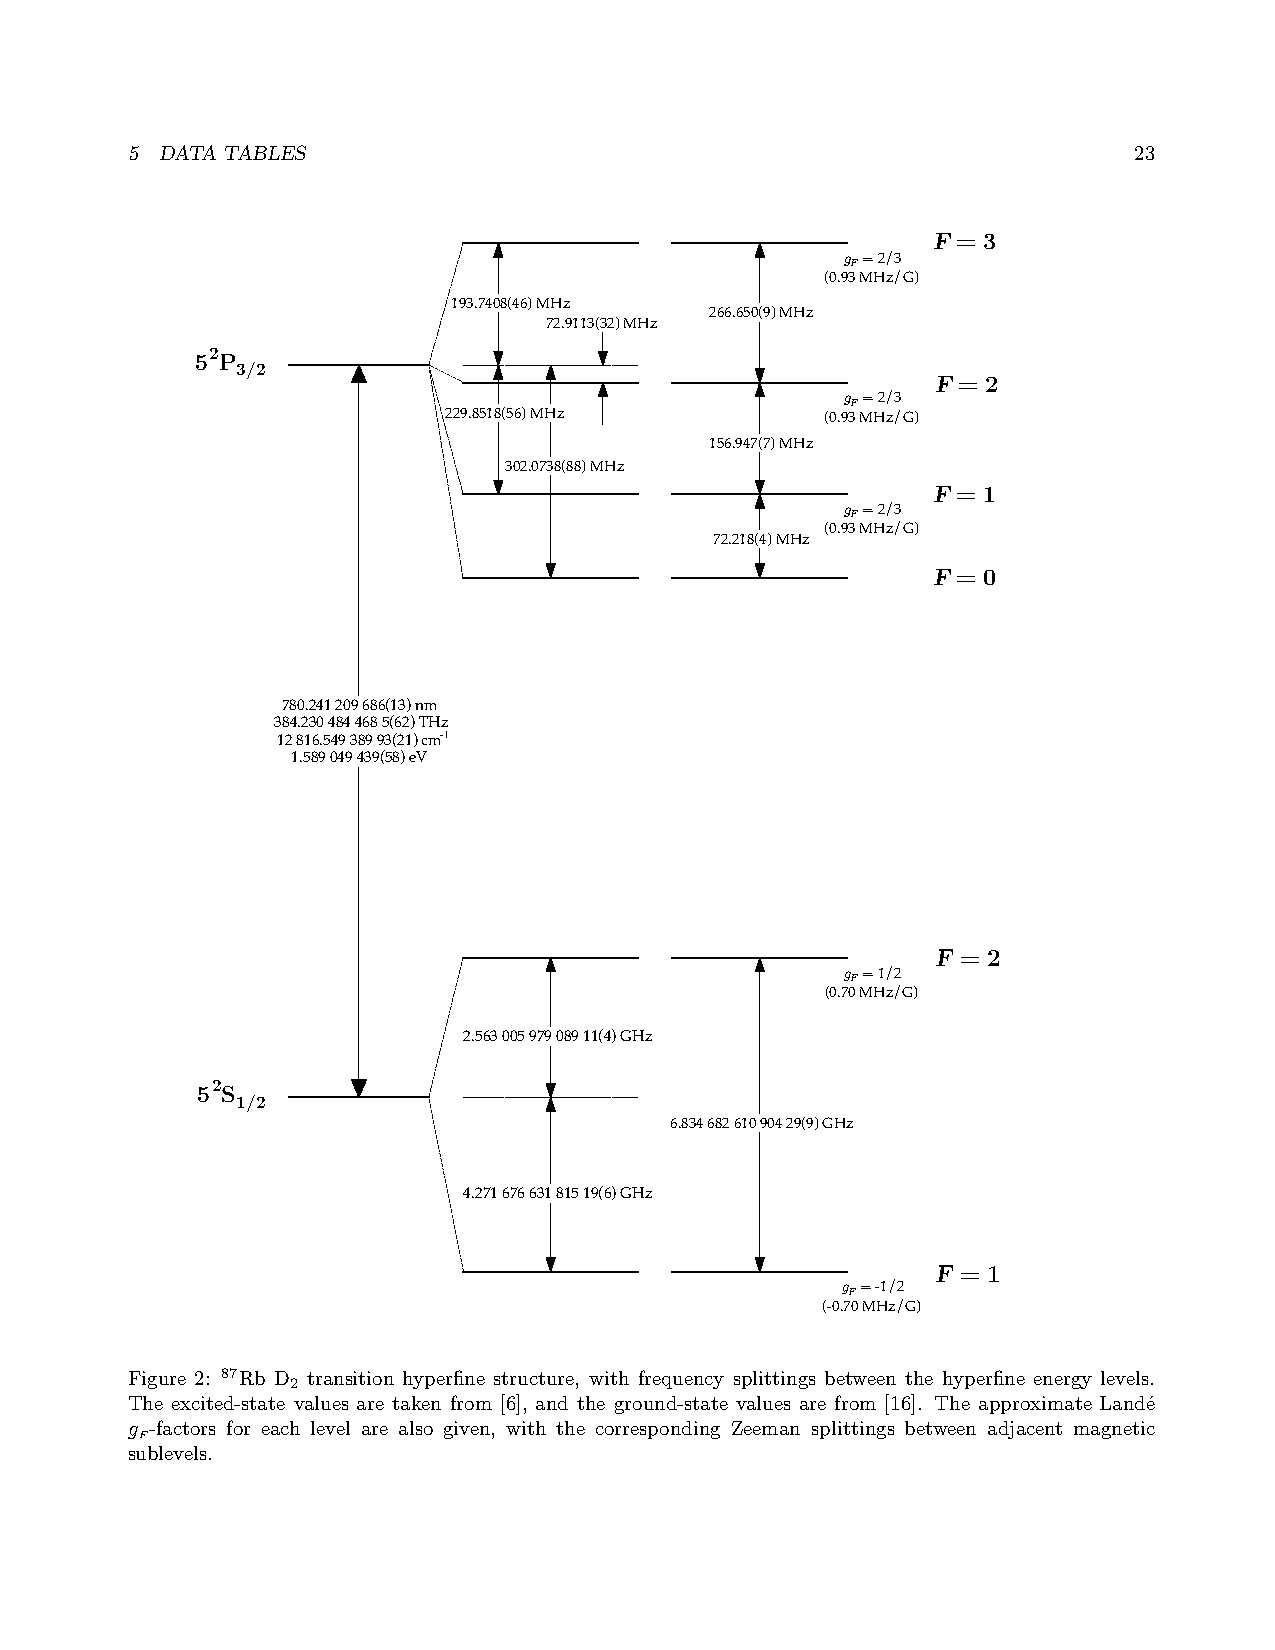
\includegraphics[width=8cm]{87D2.pdf} }}%
	\caption{Rubidium Energy Levels}%
	\label{fig:RbEnergy}%
\end{figure}

\section*{Experiment and Data}

\subsection*{Experimental Setup}


\begin{figure}%
	\centering
	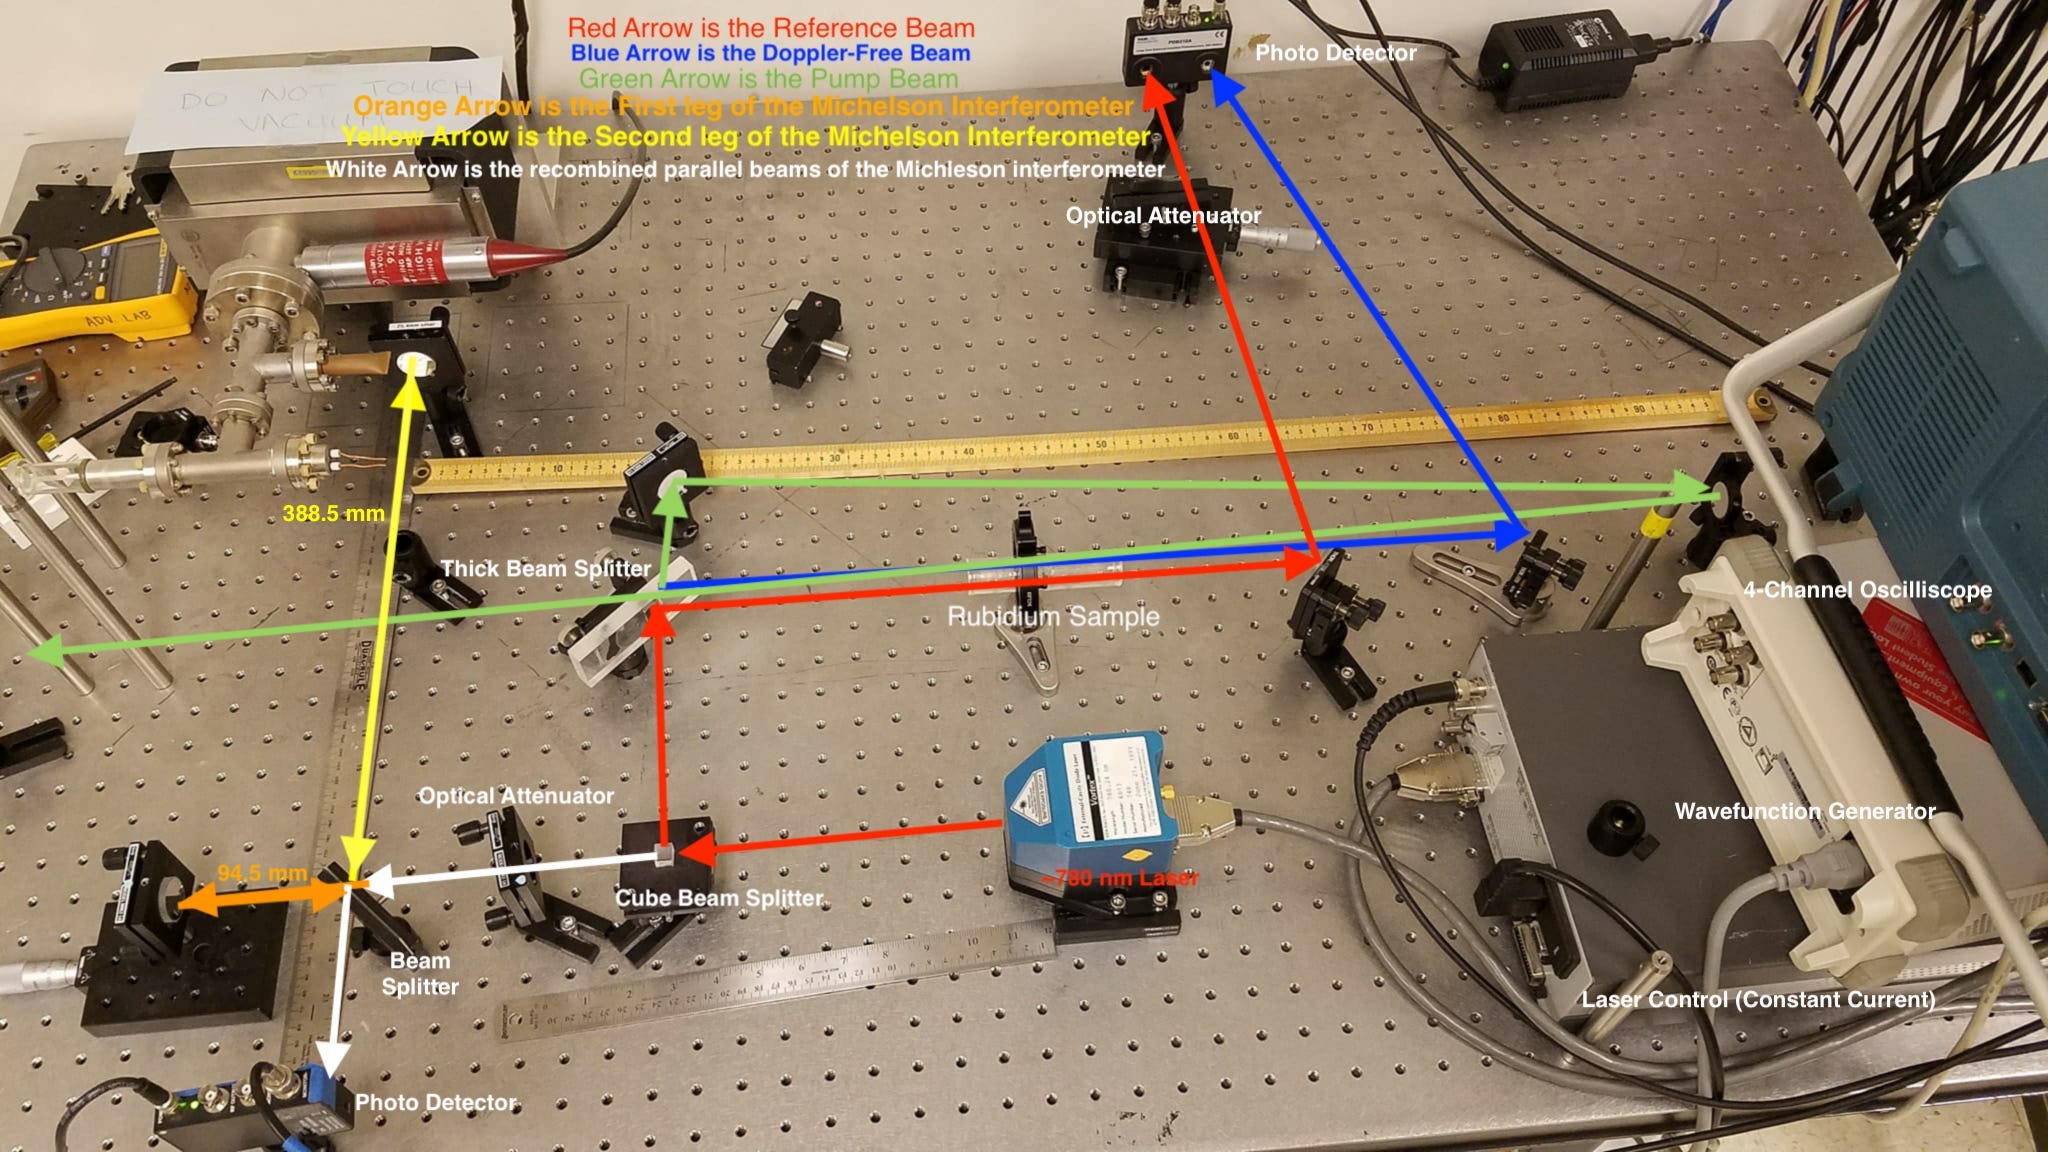
\includegraphics[width=\textwidth]{DFS_Layout.jpg}
	\caption{Experiment Layout}%
	\label{fig:Layout}%
\end{figure}

\subsection*{Results}

\subsection*{Error Analysis}

\section*{Conclusions}



\bibliographystyle{unsrt}
\bibliography{DFS_ref}

\end{document}
